\begin{frame} \frametitle{\vspace*{0.5cm}Results: Late-time evolution of the interface}
  \begin{minipage}{0.2\linewidth}
    \hfill%
    \begin{figure}
      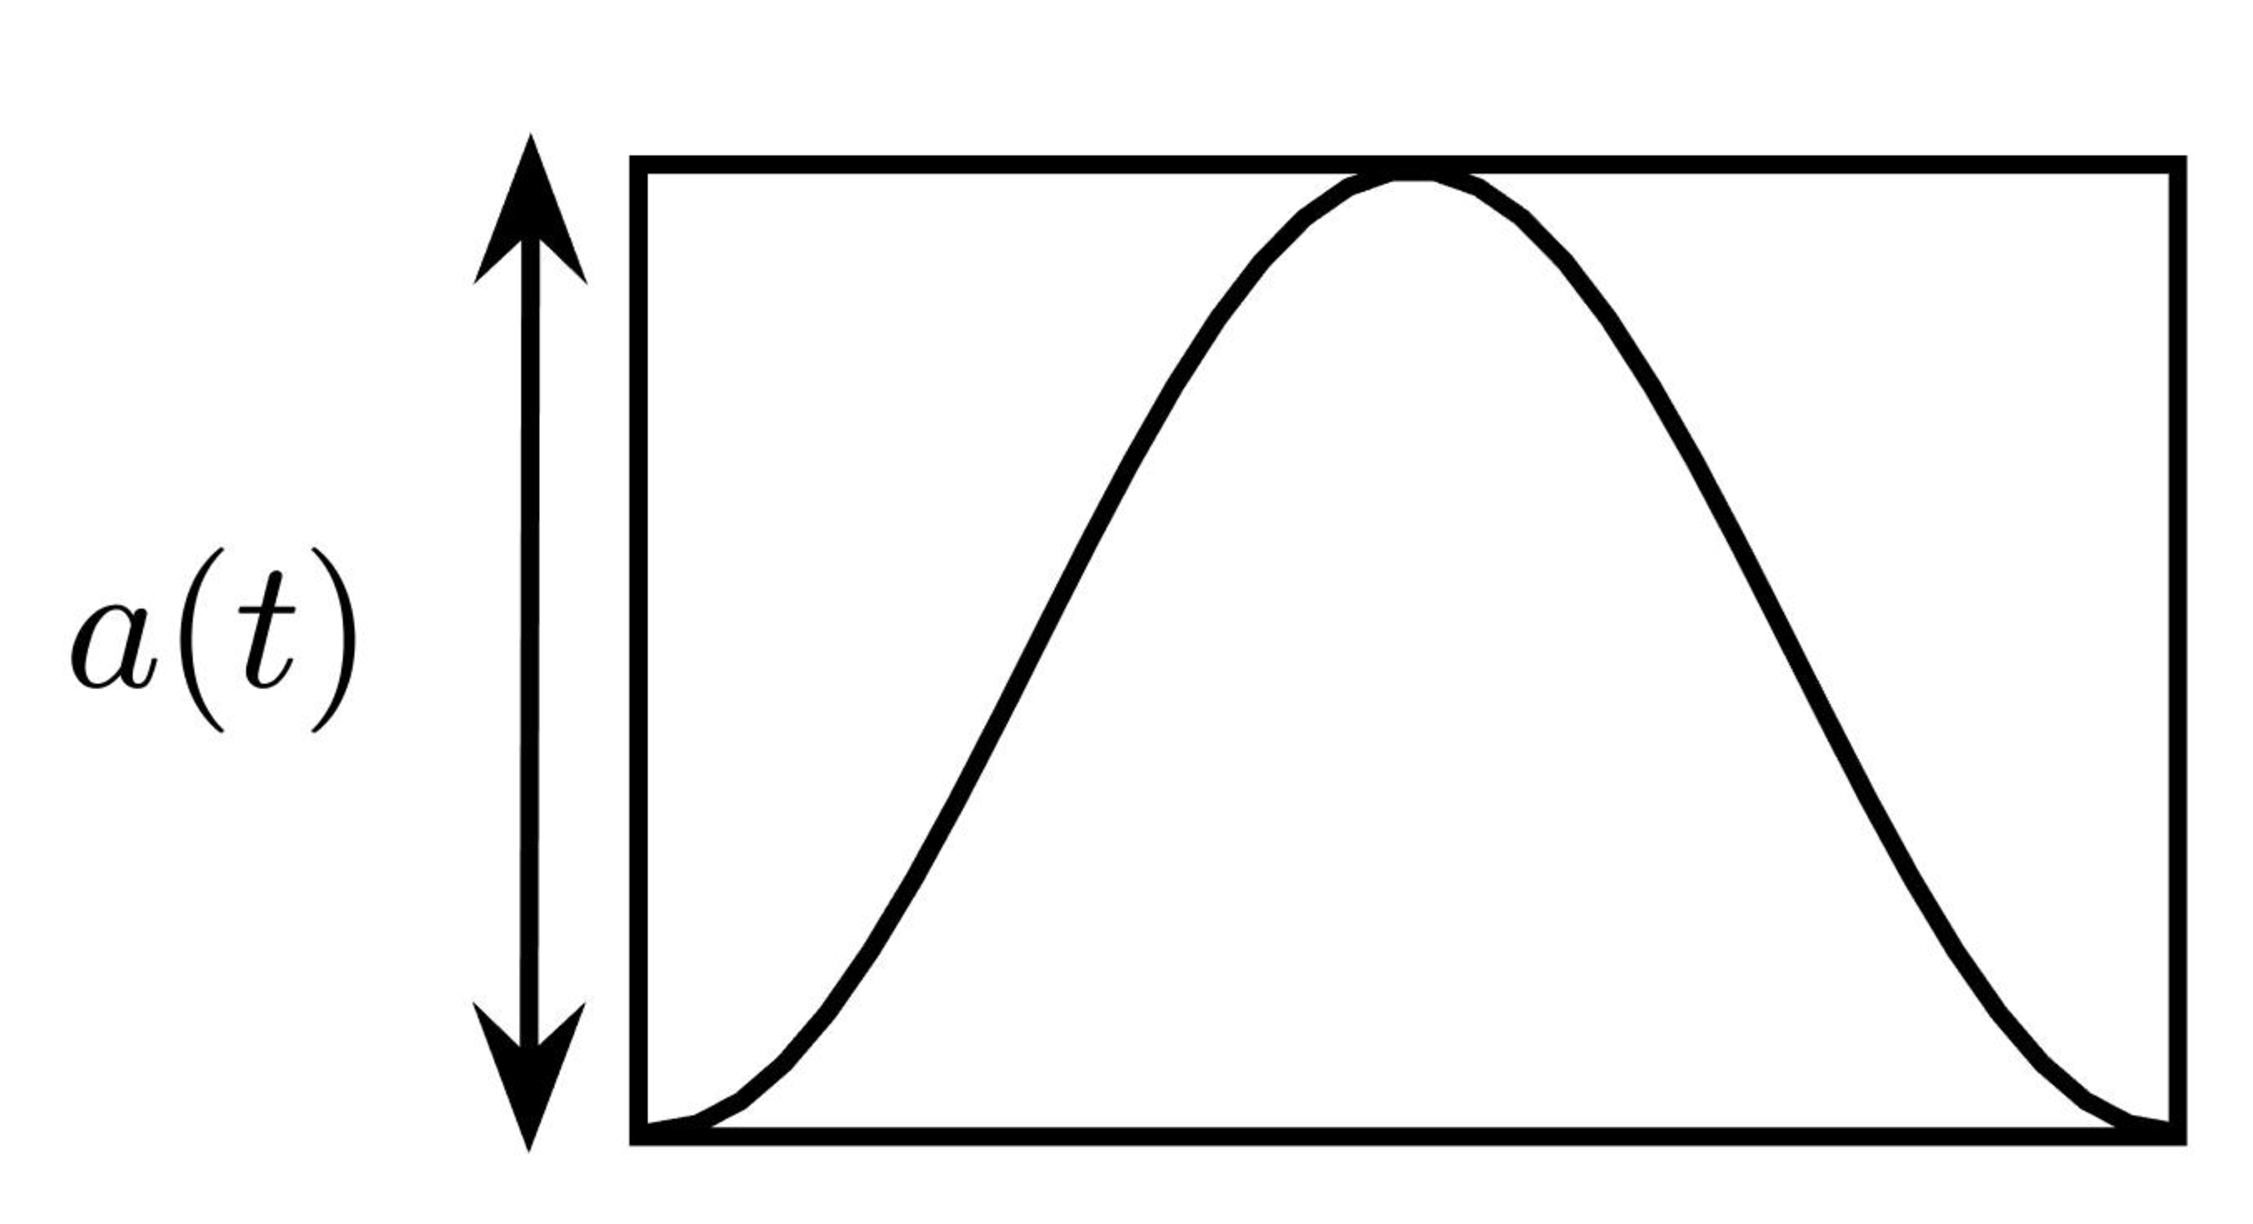
\includegraphics[height=0.18\textheight]{../figs/lung_figs/a0_schematic}%
    \end{figure}
  \end{minipage}
  \begin{minipage}{0.6\textwidth}
    \begin{figure}
      \centering%
      \hspace*{1cm}
      \begin{tikzpicture}%
        \node[anchor=south west,inner sep=0] (image) at (0,0) {%
          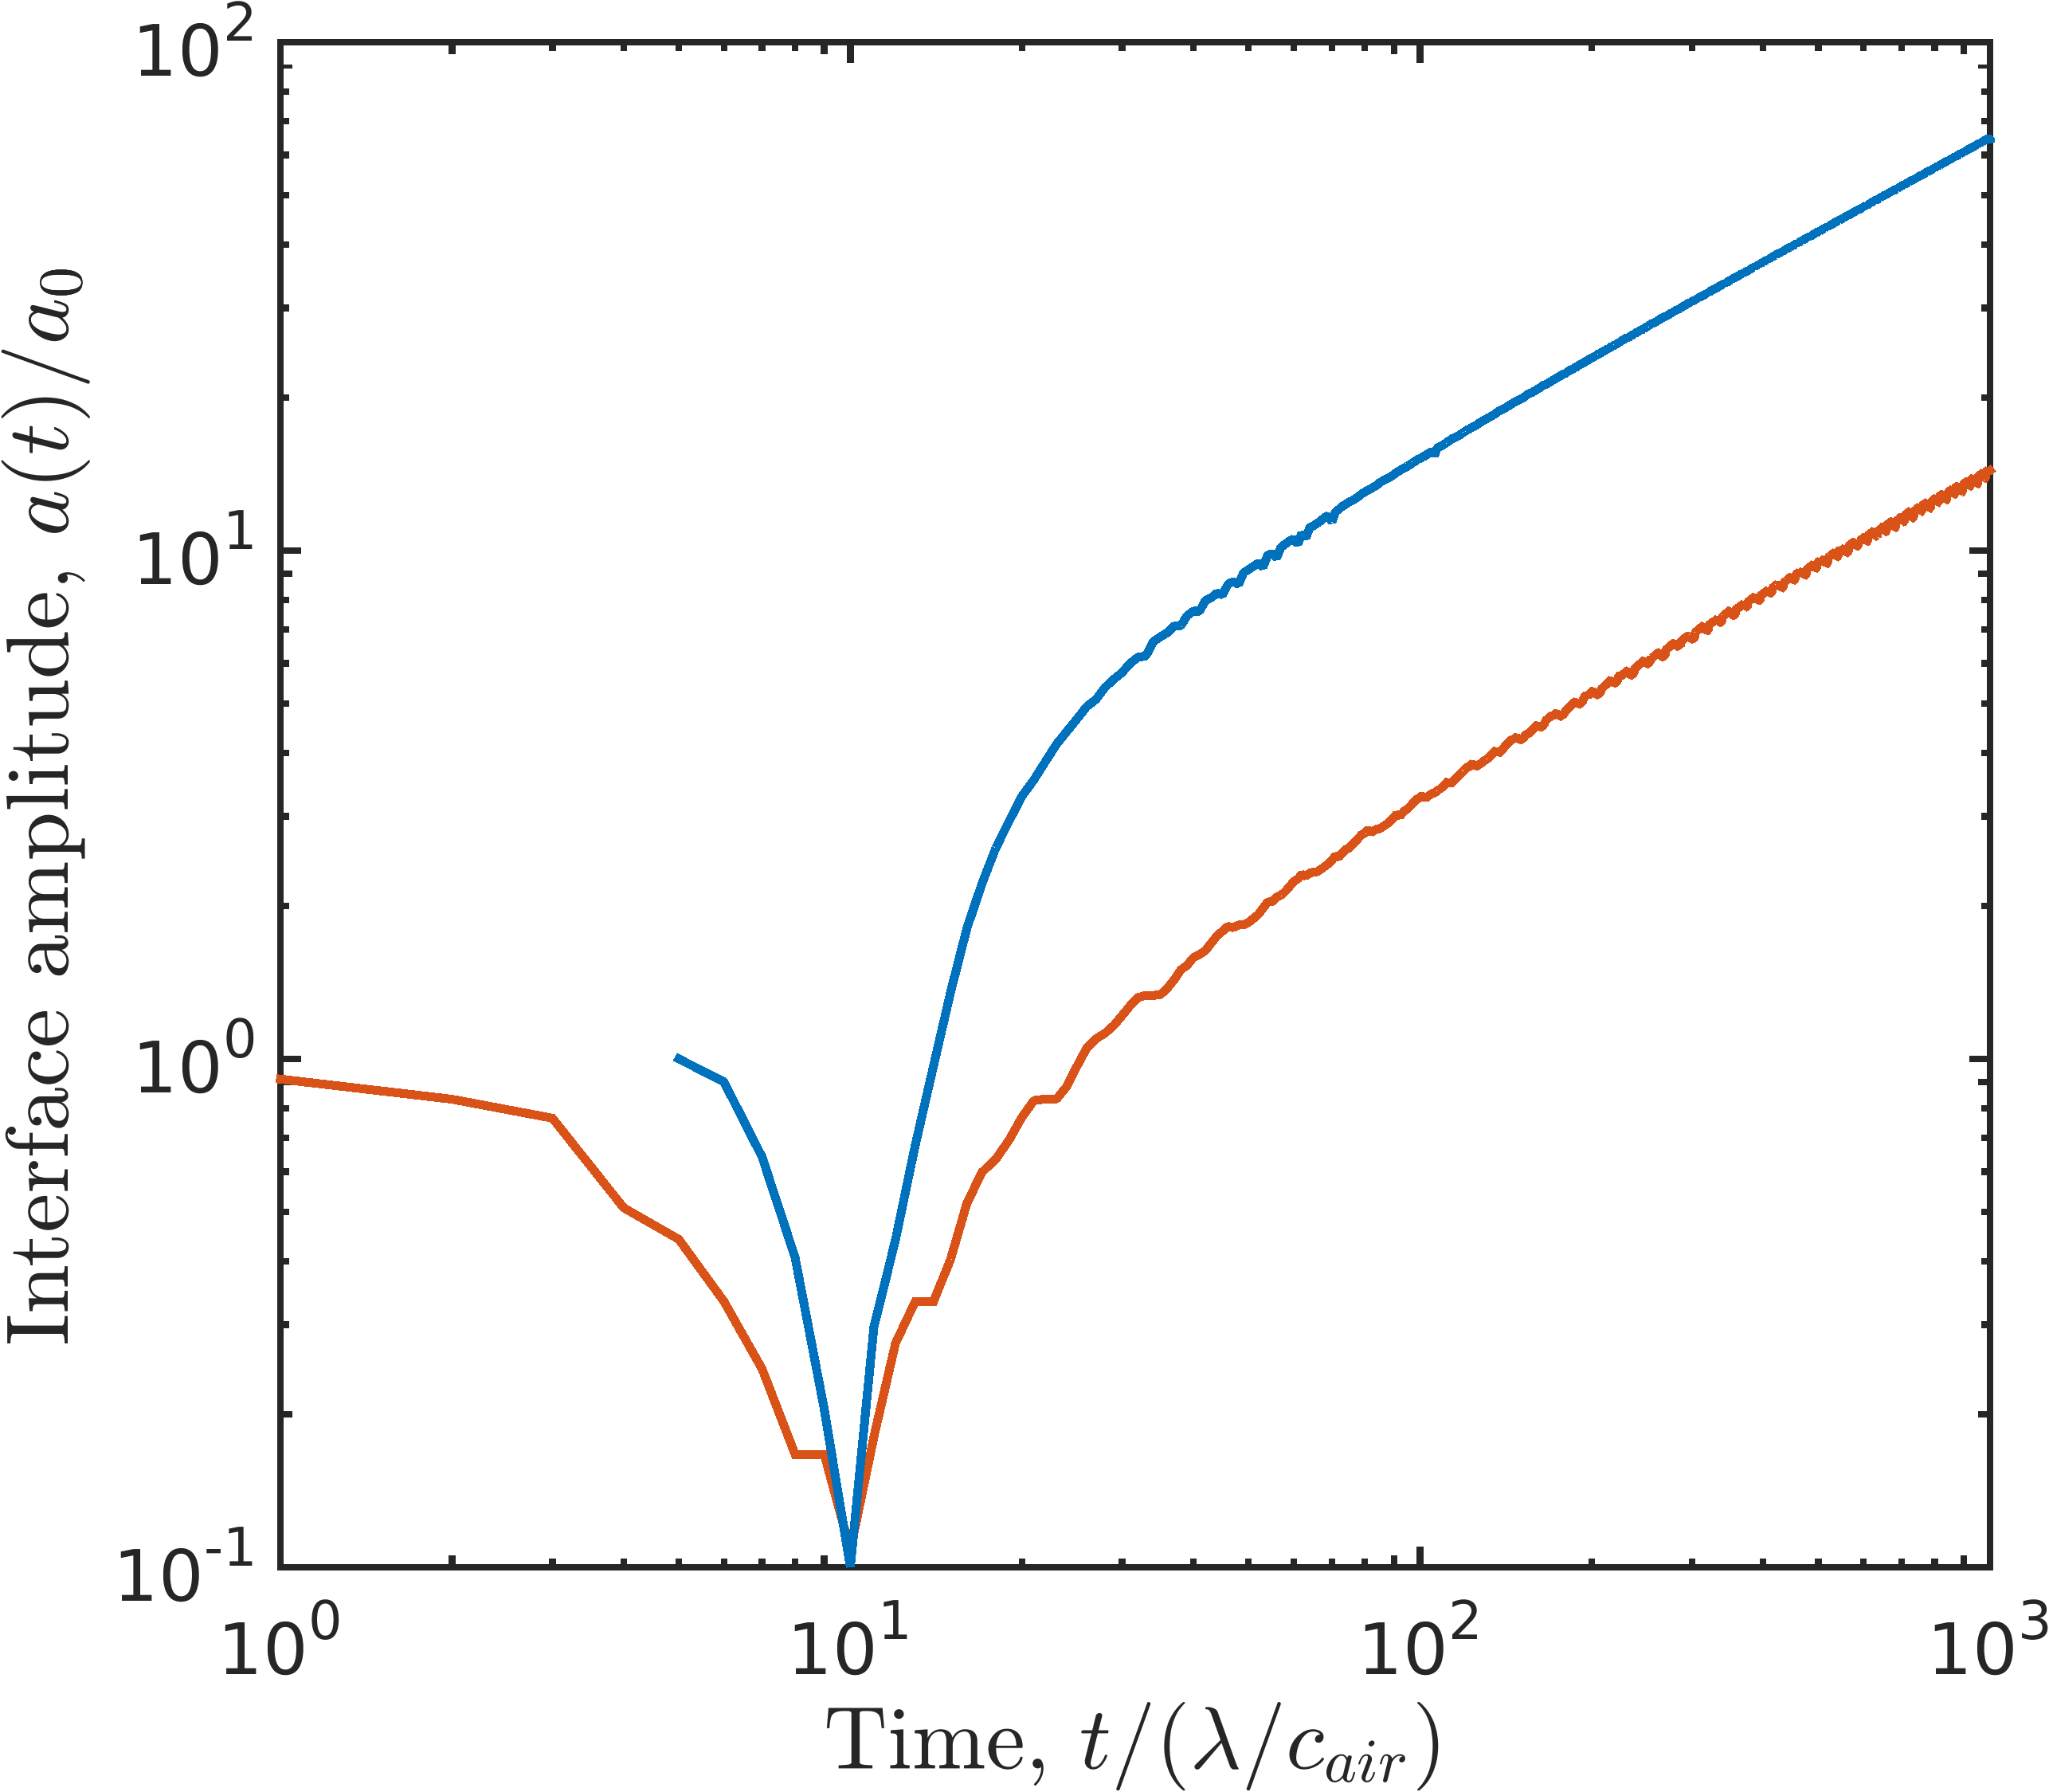
\includegraphics[width=0.9\textwidth]{../figs/lung_figs/interface_multi-amp_loglog_roe_t1000_nolines}%
        };%
        \begin{scope}[x={(image.south east)},y={(image.north west)}]%
          \node[font=\footnotesize,right] at (0.4,0.7){ $10$ MPa};%
          \node[font=\footnotesize,right] at (0.6,0.4){ $5$ MPa};%
        \end{scope}%
      \end{tikzpicture}%
    \end{figure}
  \end{minipage}
\begin{center}
    We suspect vorticity is driving this late time growth.
  \end{center}
\note{
  \begin{enumerate}
  \item If we look at this interface amplitude over a longer
    timescale, on a log-log plot we see that the growth occurs at
    similar rates for 5 and 10 MPa waves.
  \item Growth continues long after the waves are gone
  \item When vorticity is the only thing still happening in the flow
  \item We suspect vorticity is responsible for the growth.
  \end{enumerate}
}
\end{frame}
%%% Local Variables:
%%% mode: latex
%%% TeX-master: "../main"
%%% End:
